% Created by tikzDevice version 0.12.6 on 2024-04-14 13:43:38
% !TEX encoding = UTF-8 Unicode
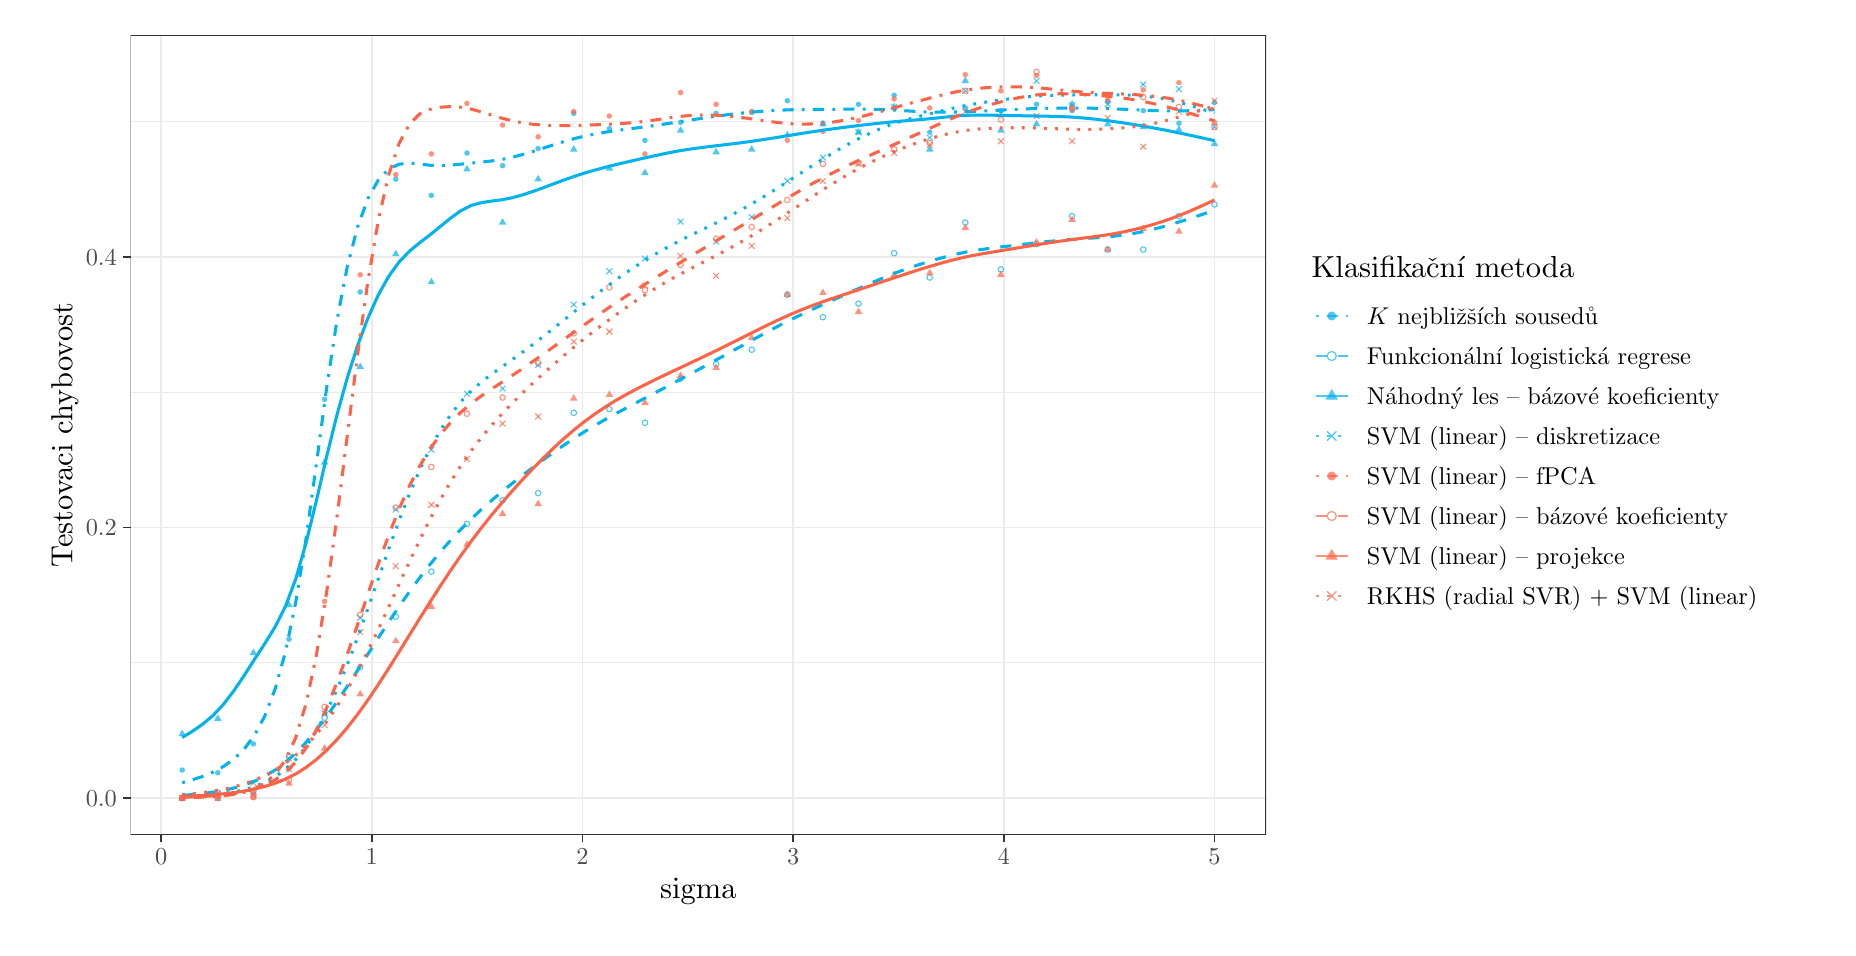
\begin{tikzpicture}[x=1pt,y=1pt]
\definecolor{fillColor}{RGB}{255,255,255}
\path[use as bounding box,fill=fillColor] (0,0) rectangle (650.43,325.21);
\begin{scope}
\path[clip] (  0.00,  0.00) rectangle (650.43,325.21);
\definecolor{drawColor}{RGB}{255,255,255}

\path[draw=drawColor,line width= 0.6pt,line join=round,line cap=round,fill=fillColor] (  0.00,  0.00) rectangle (650.43,325.21);
\end{scope}
\begin{scope}
\path[clip] ( 37.19, 33.72) rectangle (447.50,322.37);
\definecolor{fillColor}{RGB}{255,255,255}

\path[fill=fillColor] ( 37.19, 33.72) rectangle (447.50,322.37);
\definecolor{drawColor}{gray}{0.92}

\path[draw=drawColor,line width= 0.3pt,line join=round] ( 37.19, 95.74) --
	(447.50, 95.74);

\path[draw=drawColor,line width= 0.3pt,line join=round] ( 37.19,193.53) --
	(447.50,193.53);

\path[draw=drawColor,line width= 0.3pt,line join=round] ( 37.19,291.32) --
	(447.50,291.32);

\path[draw=drawColor,line width= 0.6pt,line join=round] ( 37.19, 46.84) --
	(447.50, 46.84);

\path[draw=drawColor,line width= 0.6pt,line join=round] ( 37.19,144.63) --
	(447.50,144.63);

\path[draw=drawColor,line width= 0.6pt,line join=round] ( 37.19,242.43) --
	(447.50,242.43);

\path[draw=drawColor,line width= 0.6pt,line join=round] ( 48.23, 33.72) --
	( 48.23,322.37);

\path[draw=drawColor,line width= 0.6pt,line join=round] (124.35, 33.72) --
	(124.35,322.37);

\path[draw=drawColor,line width= 0.6pt,line join=round] (200.48, 33.72) --
	(200.48,322.37);

\path[draw=drawColor,line width= 0.6pt,line join=round] (276.60, 33.72) --
	(276.60,322.37);

\path[draw=drawColor,line width= 0.6pt,line join=round] (352.72, 33.72) --
	(352.72,322.37);

\path[draw=drawColor,line width= 0.6pt,line join=round] (428.85, 33.72) --
	(428.85,322.37);
\definecolor{fillColor}{RGB}{0,178,238}

\path[fill=fillColor,fill opacity=0.70] ( 55.84, 56.95) circle (  1.00);

\path[fill=fillColor,fill opacity=0.70] ( 68.70, 55.97) circle (  1.00);

\path[fill=fillColor,fill opacity=0.70] ( 81.57, 66.40) circle (  1.00);

\path[fill=fillColor,fill opacity=0.70] ( 94.43,104.21) circle (  1.00);

\path[fill=fillColor,fill opacity=0.70] (107.29,190.92) circle (  1.00);

\path[fill=fillColor,fill opacity=0.70] (120.15,229.71) circle (  1.00);

\path[fill=fillColor,fill opacity=0.70] (133.02,270.46) circle (  1.00);

\path[fill=fillColor,fill opacity=0.70] (145.88,264.59) circle (  1.00);

\path[fill=fillColor,fill opacity=0.70] (158.74,279.91) circle (  1.00);

\path[fill=fillColor,fill opacity=0.70] (171.60,275.35) circle (  1.00);

\path[fill=fillColor,fill opacity=0.70] (184.46,281.54) circle (  1.00);

\path[fill=fillColor,fill opacity=0.70] (197.33,294.25) circle (  1.00);

\path[fill=fillColor,fill opacity=0.70] (210.19,288.71) circle (  1.00);

\path[fill=fillColor,fill opacity=0.70] (223.05,284.48) circle (  1.00);

\path[fill=fillColor,fill opacity=0.70] (235.91,290.99) circle (  1.00);

\path[fill=fillColor,fill opacity=0.70] (248.78,294.25) circle (  1.00);

\path[fill=fillColor,fill opacity=0.70] (261.64,294.58) circle (  1.00);

\path[fill=fillColor,fill opacity=0.70] (274.50,298.82) circle (  1.00);

\path[fill=fillColor,fill opacity=0.70] (287.36,290.67) circle (  1.00);

\path[fill=fillColor,fill opacity=0.70] (300.22,297.51) circle (  1.00);

\path[fill=fillColor,fill opacity=0.70] (313.09,300.77) circle (  1.00);

\path[fill=fillColor,fill opacity=0.70] (325.95,287.41) circle (  1.00);

\path[fill=fillColor,fill opacity=0.70] (338.81,296.21) circle (  1.00);

\path[fill=fillColor,fill opacity=0.70] (351.67,295.23) circle (  1.00);

\path[fill=fillColor,fill opacity=0.70] (364.54,297.51) circle (  1.00);

\path[fill=fillColor,fill opacity=0.70] (377.40,295.23) circle (  1.00);

\path[fill=fillColor,fill opacity=0.70] (390.26,298.49) circle (  1.00);

\path[fill=fillColor,fill opacity=0.70] (403.12,295.23) circle (  1.00);

\path[fill=fillColor,fill opacity=0.70] (415.99,290.67) circle (  1.00);

\path[fill=fillColor,fill opacity=0.70] (428.85,298.17) circle (  1.00);
\definecolor{drawColor}{RGB}{0,178,238}

\path[draw=drawColor,draw opacity=0.70,line width= 0.4pt,line join=round,line cap=round] ( 55.84, 46.84) circle (  1.00);

\path[draw=drawColor,draw opacity=0.70,line width= 0.4pt,line join=round,line cap=round] ( 68.70, 48.80) circle (  1.00);

\path[draw=drawColor,draw opacity=0.70,line width= 0.4pt,line join=round,line cap=round] ( 81.57, 49.45) circle (  1.00);

\path[draw=drawColor,draw opacity=0.70,line width= 0.4pt,line join=round,line cap=round] ( 94.43, 61.84) circle (  1.00);

\path[draw=drawColor,draw opacity=0.70,line width= 0.4pt,line join=round,line cap=round] (107.29, 75.85) circle (  1.00);

\path[draw=drawColor,draw opacity=0.70,line width= 0.4pt,line join=round,line cap=round] (120.15, 94.11) circle (  1.00);

\path[draw=drawColor,draw opacity=0.70,line width= 0.4pt,line join=round,line cap=round] (133.02,112.36) circle (  1.00);

\path[draw=drawColor,draw opacity=0.70,line width= 0.4pt,line join=round,line cap=round] (145.88,128.66) circle (  1.00);

\path[draw=drawColor,draw opacity=0.70,line width= 0.4pt,line join=round,line cap=round] (158.74,145.94) circle (  1.00);

\path[draw=drawColor,draw opacity=0.70,line width= 0.4pt,line join=round,line cap=round] (171.60,154.41) circle (  1.00);

\path[draw=drawColor,draw opacity=0.70,line width= 0.4pt,line join=round,line cap=round] (184.46,157.02) circle (  1.00);

\path[draw=drawColor,draw opacity=0.70,line width= 0.4pt,line join=round,line cap=round] (197.33,186.03) circle (  1.00);

\path[draw=drawColor,draw opacity=0.70,line width= 0.4pt,line join=round,line cap=round] (210.19,187.34) circle (  1.00);

\path[draw=drawColor,draw opacity=0.70,line width= 0.4pt,line join=round,line cap=round] (223.05,182.45) circle (  1.00);

\path[draw=drawColor,draw opacity=0.70,line width= 0.4pt,line join=round,line cap=round] (235.91,198.42) circle (  1.00);

\path[draw=drawColor,draw opacity=0.70,line width= 0.4pt,line join=round,line cap=round] (248.78,203.63) circle (  1.00);

\path[draw=drawColor,draw opacity=0.70,line width= 0.4pt,line join=round,line cap=round] (261.64,208.85) circle (  1.00);

\path[draw=drawColor,draw opacity=0.70,line width= 0.4pt,line join=round,line cap=round] (274.50,228.73) circle (  1.00);

\path[draw=drawColor,draw opacity=0.70,line width= 0.4pt,line join=round,line cap=round] (287.36,220.59) circle (  1.00);

\path[draw=drawColor,draw opacity=0.70,line width= 0.4pt,line join=round,line cap=round] (300.22,225.47) circle (  1.00);

\path[draw=drawColor,draw opacity=0.70,line width= 0.4pt,line join=round,line cap=round] (313.09,243.73) circle (  1.00);

\path[draw=drawColor,draw opacity=0.70,line width= 0.4pt,line join=round,line cap=round] (325.95,234.93) circle (  1.00);

\path[draw=drawColor,draw opacity=0.70,line width= 0.4pt,line join=round,line cap=round] (338.81,254.81) circle (  1.00);

\path[draw=drawColor,draw opacity=0.70,line width= 0.4pt,line join=round,line cap=round] (351.67,237.86) circle (  1.00);

\path[draw=drawColor,draw opacity=0.70,line width= 0.4pt,line join=round,line cap=round] (364.54,246.99) circle (  1.00);

\path[draw=drawColor,draw opacity=0.70,line width= 0.4pt,line join=round,line cap=round] (377.40,257.09) circle (  1.00);

\path[draw=drawColor,draw opacity=0.70,line width= 0.4pt,line join=round,line cap=round] (390.26,245.03) circle (  1.00);

\path[draw=drawColor,draw opacity=0.70,line width= 0.4pt,line join=round,line cap=round] (403.12,245.03) circle (  1.00);

\path[draw=drawColor,draw opacity=0.70,line width= 0.4pt,line join=round,line cap=round] (415.99,257.09) circle (  1.00);

\path[draw=drawColor,draw opacity=0.70,line width= 0.4pt,line join=round,line cap=round] (428.85,261.33) circle (  1.00);

\path[fill=fillColor,fill opacity=0.70] ( 55.84, 71.54) --
	( 57.19, 69.21) --
	( 54.50, 69.21) --
	cycle;

\path[fill=fillColor,fill opacity=0.70] ( 68.70, 77.08) --
	( 70.05, 74.75) --
	( 67.36, 74.75) --
	cycle;

\path[fill=fillColor,fill opacity=0.70] ( 81.57,100.88) --
	( 82.91, 98.55) --
	( 80.22, 98.55) --
	cycle;

\path[fill=fillColor,fill opacity=0.70] ( 94.43,118.15) --
	( 95.77,115.82) --
	( 93.08,115.82) --
	cycle;

\path[fill=fillColor,fill opacity=0.70] (107.29,169.66) --
	(108.64,167.33) --
	(105.95,167.33) --
	cycle;

\path[fill=fillColor,fill opacity=0.70] (120.15,204.21) --
	(121.50,201.88) --
	(118.81,201.88) --
	cycle;

\path[fill=fillColor,fill opacity=0.70] (133.02,244.96) --
	(134.36,242.63) --
	(131.67,242.63) --
	cycle;

\path[fill=fillColor,fill opacity=0.70] (145.88,234.85) --
	(147.22,232.52) --
	(144.53,232.52) --
	cycle;

\path[fill=fillColor,fill opacity=0.70] (158.74,275.60) --
	(160.08,273.27) --
	(157.40,273.27) --
	cycle;

\path[fill=fillColor,fill opacity=0.70] (171.60,256.36) --
	(172.95,254.04) --
	(170.26,254.04) --
	cycle;

\path[fill=fillColor,fill opacity=0.70] (184.46,272.01) --
	(185.81,269.68) --
	(183.12,269.68) --
	cycle;

\path[fill=fillColor,fill opacity=0.70] (197.33,282.77) --
	(198.67,280.44) --
	(195.98,280.44) --
	cycle;

\path[fill=fillColor,fill opacity=0.70] (210.19,275.92) --
	(211.53,273.59) --
	(208.84,273.59) --
	cycle;

\path[fill=fillColor,fill opacity=0.70] (223.05,274.29) --
	(224.40,271.96) --
	(221.71,271.96) --
	cycle;

\path[fill=fillColor,fill opacity=0.70] (235.91,289.61) --
	(237.26,287.28) --
	(234.57,287.28) --
	cycle;

\path[fill=fillColor,fill opacity=0.70] (248.78,281.79) --
	(250.12,279.46) --
	(247.43,279.46) --
	cycle;

\path[fill=fillColor,fill opacity=0.70] (261.64,282.77) --
	(262.98,280.44) --
	(260.29,280.44) --
	cycle;

\path[fill=fillColor,fill opacity=0.70] (274.50,287.98) --
	(275.84,285.66) --
	(273.16,285.66) --
	cycle;

\path[fill=fillColor,fill opacity=0.70] (287.36,291.90) --
	(288.71,289.57) --
	(286.02,289.57) --
	cycle;

\path[fill=fillColor,fill opacity=0.70] (300.22,288.96) --
	(301.57,286.63) --
	(298.88,286.63) --
	cycle;

\path[fill=fillColor,fill opacity=0.70] (313.09,298.09) --
	(314.43,295.76) --
	(311.74,295.76) --
	cycle;

\path[fill=fillColor,fill opacity=0.70] (325.95,282.77) --
	(327.29,280.44) --
	(324.61,280.44) --
	cycle;

\path[fill=fillColor,fill opacity=0.70] (338.81,307.54) --
	(340.16,305.21) --
	(337.47,305.21) --
	cycle;

\path[fill=fillColor,fill opacity=0.70] (351.67,289.61) --
	(353.02,287.28) --
	(350.33,287.28) --
	cycle;

\path[fill=fillColor,fill opacity=0.70] (364.54,291.90) --
	(365.88,289.57) --
	(363.19,289.57) --
	cycle;

\path[fill=fillColor,fill opacity=0.70] (377.40,299.07) --
	(378.74,296.74) --
	(376.05,296.74) --
	cycle;

\path[fill=fillColor,fill opacity=0.70] (390.26,291.90) --
	(391.61,289.57) --
	(388.92,289.57) --
	cycle;

\path[fill=fillColor,fill opacity=0.70] (403.12,290.92) --
	(404.47,288.59) --
	(401.78,288.59) --
	cycle;

\path[fill=fillColor,fill opacity=0.70] (415.99,289.94) --
	(417.33,287.61) --
	(414.64,287.61) --
	cycle;

\path[fill=fillColor,fill opacity=0.70] (428.85,284.72) --
	(430.19,282.40) --
	(427.50,282.40) --
	cycle;

\path[draw=drawColor,draw opacity=0.70,line width= 0.4pt,line join=round,line cap=round] ( 54.84, 45.84) -- ( 56.84, 47.84);

\path[draw=drawColor,draw opacity=0.70,line width= 0.4pt,line join=round,line cap=round] ( 54.84, 47.84) -- ( 56.84, 45.84);

\path[draw=drawColor,draw opacity=0.70,line width= 0.4pt,line join=round,line cap=round] ( 67.71, 45.84) -- ( 69.70, 47.84);

\path[draw=drawColor,draw opacity=0.70,line width= 0.4pt,line join=round,line cap=round] ( 67.71, 47.84) -- ( 69.70, 45.84);

\path[draw=drawColor,draw opacity=0.70,line width= 0.4pt,line join=round,line cap=round] ( 80.57, 47.15) -- ( 82.56, 49.14);

\path[draw=drawColor,draw opacity=0.70,line width= 0.4pt,line join=round,line cap=round] ( 80.57, 49.14) -- ( 82.56, 47.15);

\path[draw=drawColor,draw opacity=0.70,line width= 0.4pt,line join=round,line cap=round] ( 93.43, 56.27) -- ( 95.43, 58.27);

\path[draw=drawColor,draw opacity=0.70,line width= 0.4pt,line join=round,line cap=round] ( 93.43, 58.27) -- ( 95.43, 56.27);

\path[draw=drawColor,draw opacity=0.70,line width= 0.4pt,line join=round,line cap=round] (106.29, 76.49) -- (108.29, 78.48);

\path[draw=drawColor,draw opacity=0.70,line width= 0.4pt,line join=round,line cap=round] (106.29, 78.48) -- (108.29, 76.49);

\path[draw=drawColor,draw opacity=0.70,line width= 0.4pt,line join=round,line cap=round] (119.16,111.04) -- (121.15,113.03);

\path[draw=drawColor,draw opacity=0.70,line width= 0.4pt,line join=round,line cap=round] (119.16,113.03) -- (121.15,111.04);

\path[draw=drawColor,draw opacity=0.70,line width= 0.4pt,line join=round,line cap=round] (132.02,150.15) -- (134.01,152.15);

\path[draw=drawColor,draw opacity=0.70,line width= 0.4pt,line join=round,line cap=round] (132.02,152.15) -- (134.01,150.15);

\path[draw=drawColor,draw opacity=0.70,line width= 0.4pt,line join=round,line cap=round] (144.88,171.67) -- (146.88,173.67);

\path[draw=drawColor,draw opacity=0.70,line width= 0.4pt,line join=round,line cap=round] (144.88,173.67) -- (146.88,171.67);

\path[draw=drawColor,draw opacity=0.70,line width= 0.4pt,line join=round,line cap=round] (157.74,191.88) -- (159.74,193.88);

\path[draw=drawColor,draw opacity=0.70,line width= 0.4pt,line join=round,line cap=round] (157.74,193.88) -- (159.74,191.88);

\path[draw=drawColor,draw opacity=0.70,line width= 0.4pt,line join=round,line cap=round] (170.60,193.83) -- (172.60,195.83);

\path[draw=drawColor,draw opacity=0.70,line width= 0.4pt,line join=round,line cap=round] (170.60,195.83) -- (172.60,193.83);

\path[draw=drawColor,draw opacity=0.70,line width= 0.4pt,line join=round,line cap=round] (183.47,202.31) -- (185.46,204.31);

\path[draw=drawColor,draw opacity=0.70,line width= 0.4pt,line join=round,line cap=round] (183.47,204.31) -- (185.46,202.31);

\path[draw=drawColor,draw opacity=0.70,line width= 0.4pt,line join=round,line cap=round] (196.33,224.15) -- (198.33,226.15);

\path[draw=drawColor,draw opacity=0.70,line width= 0.4pt,line join=round,line cap=round] (196.33,226.15) -- (198.33,224.15);

\path[draw=drawColor,draw opacity=0.70,line width= 0.4pt,line join=round,line cap=round] (209.19,236.21) -- (211.19,238.21);

\path[draw=drawColor,draw opacity=0.70,line width= 0.4pt,line join=round,line cap=round] (209.19,238.21) -- (211.19,236.21);

\path[draw=drawColor,draw opacity=0.70,line width= 0.4pt,line join=round,line cap=round] (222.05,240.77) -- (224.05,242.77);

\path[draw=drawColor,draw opacity=0.70,line width= 0.4pt,line join=round,line cap=round] (222.05,242.77) -- (224.05,240.77);

\path[draw=drawColor,draw opacity=0.70,line width= 0.4pt,line join=round,line cap=round] (234.92,254.14) -- (236.91,256.14);

\path[draw=drawColor,draw opacity=0.70,line width= 0.4pt,line join=round,line cap=round] (234.92,256.14) -- (236.91,254.14);

\path[draw=drawColor,draw opacity=0.70,line width= 0.4pt,line join=round,line cap=round] (247.78,246.97) -- (249.77,248.96);

\path[draw=drawColor,draw opacity=0.70,line width= 0.4pt,line join=round,line cap=round] (247.78,248.96) -- (249.77,246.97);

\path[draw=drawColor,draw opacity=0.70,line width= 0.4pt,line join=round,line cap=round] (260.64,255.77) -- (262.64,257.77);

\path[draw=drawColor,draw opacity=0.70,line width= 0.4pt,line join=round,line cap=round] (260.64,257.77) -- (262.64,255.77);

\path[draw=drawColor,draw opacity=0.70,line width= 0.4pt,line join=round,line cap=round] (273.50,268.81) -- (275.50,270.81);

\path[draw=drawColor,draw opacity=0.70,line width= 0.4pt,line join=round,line cap=round] (273.50,270.81) -- (275.50,268.81);

\path[draw=drawColor,draw opacity=0.70,line width= 0.4pt,line join=round,line cap=round] (286.36,277.28) -- (288.36,279.28);

\path[draw=drawColor,draw opacity=0.70,line width= 0.4pt,line join=round,line cap=round] (286.36,279.28) -- (288.36,277.28);

\path[draw=drawColor,draw opacity=0.70,line width= 0.4pt,line join=round,line cap=round] (299.23,286.41) -- (301.22,288.41);

\path[draw=drawColor,draw opacity=0.70,line width= 0.4pt,line join=round,line cap=round] (299.23,288.41) -- (301.22,286.41);

\path[draw=drawColor,draw opacity=0.70,line width= 0.4pt,line join=round,line cap=round] (312.09,295.54) -- (314.09,297.53);

\path[draw=drawColor,draw opacity=0.70,line width= 0.4pt,line join=round,line cap=round] (312.09,297.53) -- (314.09,295.54);

\path[draw=drawColor,draw opacity=0.70,line width= 0.4pt,line join=round,line cap=round] (324.95,284.46) -- (326.95,286.45);

\path[draw=drawColor,draw opacity=0.70,line width= 0.4pt,line join=round,line cap=round] (324.95,286.45) -- (326.95,284.46);

\path[draw=drawColor,draw opacity=0.70,line width= 0.4pt,line join=round,line cap=round] (337.81,301.41) -- (339.81,303.40);

\path[draw=drawColor,draw opacity=0.70,line width= 0.4pt,line join=round,line cap=round] (337.81,303.40) -- (339.81,301.41);

\path[draw=drawColor,draw opacity=0.70,line width= 0.4pt,line join=round,line cap=round] (350.68,293.26) -- (352.67,295.25);

\path[draw=drawColor,draw opacity=0.70,line width= 0.4pt,line join=round,line cap=round] (350.68,295.25) -- (352.67,293.26);

\path[draw=drawColor,draw opacity=0.70,line width= 0.4pt,line join=round,line cap=round] (363.54,304.99) -- (365.53,306.99);

\path[draw=drawColor,draw opacity=0.70,line width= 0.4pt,line join=round,line cap=round] (363.54,306.99) -- (365.53,304.99);

\path[draw=drawColor,draw opacity=0.70,line width= 0.4pt,line join=round,line cap=round] (376.40,296.19) -- (378.40,298.19);

\path[draw=drawColor,draw opacity=0.70,line width= 0.4pt,line join=round,line cap=round] (376.40,298.19) -- (378.40,296.19);

\path[draw=drawColor,draw opacity=0.70,line width= 0.4pt,line join=round,line cap=round] (389.26,296.52) -- (391.26,298.51);

\path[draw=drawColor,draw opacity=0.70,line width= 0.4pt,line join=round,line cap=round] (389.26,298.51) -- (391.26,296.52);

\path[draw=drawColor,draw opacity=0.70,line width= 0.4pt,line join=round,line cap=round] (402.12,303.69) -- (404.12,305.68);

\path[draw=drawColor,draw opacity=0.70,line width= 0.4pt,line join=round,line cap=round] (402.12,305.68) -- (404.12,303.69);

\path[draw=drawColor,draw opacity=0.70,line width= 0.4pt,line join=round,line cap=round] (414.99,302.06) -- (416.98,304.05);

\path[draw=drawColor,draw opacity=0.70,line width= 0.4pt,line join=round,line cap=round] (414.99,304.05) -- (416.98,302.06);

\path[draw=drawColor,draw opacity=0.70,line width= 0.4pt,line join=round,line cap=round] (427.85,288.37) -- (429.85,290.36);

\path[draw=drawColor,draw opacity=0.70,line width= 0.4pt,line join=round,line cap=round] (427.85,290.36) -- (429.85,288.37);
\definecolor{fillColor}{RGB}{255,99,71}

\path[fill=fillColor,fill opacity=0.70] ( 55.84, 46.84) circle (  1.00);

\path[fill=fillColor,fill opacity=0.70] ( 68.70, 46.84) circle (  1.00);

\path[fill=fillColor,fill opacity=0.70] ( 81.57, 47.17) circle (  1.00);

\path[fill=fillColor,fill opacity=0.70] ( 94.43, 57.60) circle (  1.00);

\path[fill=fillColor,fill opacity=0.70] (107.29,117.90) circle (  1.00);

\path[fill=fillColor,fill opacity=0.70] (120.15,235.91) circle (  1.00);

\path[fill=fillColor,fill opacity=0.70] (133.02,272.09) circle (  1.00);

\path[fill=fillColor,fill opacity=0.70] (145.88,279.59) circle (  1.00);

\path[fill=fillColor,fill opacity=0.70] (158.74,297.84) circle (  1.00);

\path[fill=fillColor,fill opacity=0.70] (171.60,290.02) circle (  1.00);

\path[fill=fillColor,fill opacity=0.70] (184.46,285.78) circle (  1.00);

\path[fill=fillColor,fill opacity=0.70] (197.33,294.91) circle (  1.00);

\path[fill=fillColor,fill opacity=0.70] (210.19,293.28) circle (  1.00);

\path[fill=fillColor,fill opacity=0.70] (223.05,279.59) circle (  1.00);

\path[fill=fillColor,fill opacity=0.70] (235.91,301.75) circle (  1.00);

\path[fill=fillColor,fill opacity=0.70] (248.78,297.51) circle (  1.00);

\path[fill=fillColor,fill opacity=0.70] (261.64,294.91) circle (  1.00);

\path[fill=fillColor,fill opacity=0.70] (274.50,284.48) circle (  1.00);

\path[fill=fillColor,fill opacity=0.70] (287.36,287.74) circle (  1.00);

\path[fill=fillColor,fill opacity=0.70] (300.22,291.65) circle (  1.00);

\path[fill=fillColor,fill opacity=0.70] (313.09,299.47) circle (  1.00);

\path[fill=fillColor,fill opacity=0.70] (325.95,296.21) circle (  1.00);

\path[fill=fillColor,fill opacity=0.70] (338.81,308.27) circle (  1.00);

\path[fill=fillColor,fill opacity=0.70] (351.67,302.40) circle (  1.00);

\path[fill=fillColor,fill opacity=0.70] (364.54,307.95) circle (  1.00);

\path[fill=fillColor,fill opacity=0.70] (377.40,296.21) circle (  1.00);

\path[fill=fillColor,fill opacity=0.70] (390.26,299.14) circle (  1.00);

\path[fill=fillColor,fill opacity=0.70] (403.12,302.73) circle (  1.00);

\path[fill=fillColor,fill opacity=0.70] (415.99,305.34) circle (  1.00);

\path[fill=fillColor,fill opacity=0.70] (428.85,290.99) circle (  1.00);
\definecolor{drawColor}{RGB}{255,99,71}

\path[draw=drawColor,draw opacity=0.70,line width= 0.4pt,line join=round,line cap=round] ( 55.84, 46.84) circle (  1.00);

\path[draw=drawColor,draw opacity=0.70,line width= 0.4pt,line join=round,line cap=round] ( 68.70, 46.84) circle (  1.00);

\path[draw=drawColor,draw opacity=0.70,line width= 0.4pt,line join=round,line cap=round] ( 81.57, 47.17) circle (  1.00);

\path[draw=drawColor,draw opacity=0.70,line width= 0.4pt,line join=round,line cap=round] ( 94.43, 53.36) circle (  1.00);

\path[draw=drawColor,draw opacity=0.70,line width= 0.4pt,line join=round,line cap=round] (107.29, 79.77) circle (  1.00);

\path[draw=drawColor,draw opacity=0.70,line width= 0.4pt,line join=round,line cap=round] (120.15,113.01) circle (  1.00);

\path[draw=drawColor,draw opacity=0.70,line width= 0.4pt,line join=round,line cap=round] (133.02,151.80) circle (  1.00);

\path[draw=drawColor,draw opacity=0.70,line width= 0.4pt,line join=round,line cap=round] (145.88,166.47) circle (  1.00);

\path[draw=drawColor,draw opacity=0.70,line width= 0.4pt,line join=round,line cap=round] (158.74,185.71) circle (  1.00);

\path[draw=drawColor,draw opacity=0.70,line width= 0.4pt,line join=round,line cap=round] (171.60,191.57) circle (  1.00);

\path[draw=drawColor,draw opacity=0.70,line width= 0.4pt,line join=round,line cap=round] (184.46,203.96) circle (  1.00);

\path[draw=drawColor,draw opacity=0.70,line width= 0.4pt,line join=round,line cap=round] (197.33,214.72) circle (  1.00);

\path[draw=drawColor,draw opacity=0.70,line width= 0.4pt,line join=round,line cap=round] (210.19,231.34) circle (  1.00);

\path[draw=drawColor,draw opacity=0.70,line width= 0.4pt,line join=round,line cap=round] (223.05,230.36) circle (  1.00);

\path[draw=drawColor,draw opacity=0.70,line width= 0.4pt,line join=round,line cap=round] (235.91,239.49) circle (  1.00);

\path[draw=drawColor,draw opacity=0.70,line width= 0.4pt,line join=round,line cap=round] (248.78,248.94) circle (  1.00);

\path[draw=drawColor,draw opacity=0.70,line width= 0.4pt,line join=round,line cap=round] (261.64,253.18) circle (  1.00);

\path[draw=drawColor,draw opacity=0.70,line width= 0.4pt,line join=round,line cap=round] (274.50,262.96) circle (  1.00);

\path[draw=drawColor,draw opacity=0.70,line width= 0.4pt,line join=round,line cap=round] (287.36,276.00) circle (  1.00);

\path[draw=drawColor,draw opacity=0.70,line width= 0.4pt,line join=round,line cap=round] (300.22,276.33) circle (  1.00);

\path[draw=drawColor,draw opacity=0.70,line width= 0.4pt,line join=round,line cap=round] (313.09,281.22) circle (  1.00);

\path[draw=drawColor,draw opacity=0.70,line width= 0.4pt,line join=round,line cap=round] (325.95,283.50) circle (  1.00);

\path[draw=drawColor,draw opacity=0.70,line width= 0.4pt,line join=round,line cap=round] (338.81,302.40) circle (  1.00);

\path[draw=drawColor,draw opacity=0.70,line width= 0.4pt,line join=round,line cap=round] (351.67,291.97) circle (  1.00);

\path[draw=drawColor,draw opacity=0.70,line width= 0.4pt,line join=round,line cap=round] (364.54,309.25) circle (  1.00);

\path[draw=drawColor,draw opacity=0.70,line width= 0.4pt,line join=round,line cap=round] (377.40,295.88) circle (  1.00);

\path[draw=drawColor,draw opacity=0.70,line width= 0.4pt,line join=round,line cap=round] (390.26,300.77) circle (  1.00);

\path[draw=drawColor,draw opacity=0.70,line width= 0.4pt,line join=round,line cap=round] (403.12,300.12) circle (  1.00);

\path[draw=drawColor,draw opacity=0.70,line width= 0.4pt,line join=round,line cap=round] (415.99,296.54) circle (  1.00);

\path[draw=drawColor,draw opacity=0.70,line width= 0.4pt,line join=round,line cap=round] (428.85,289.37) circle (  1.00);

\path[fill=fillColor,fill opacity=0.70] ( 55.84, 48.39) --
	( 57.19, 46.07) --
	( 54.50, 46.07) --
	cycle;

\path[fill=fillColor,fill opacity=0.70] ( 68.70, 49.37) --
	( 70.05, 47.04) --
	( 67.36, 47.04) --
	cycle;

\path[fill=fillColor,fill opacity=0.70] ( 81.57, 50.35) --
	( 82.91, 48.02) --
	( 80.22, 48.02) --
	cycle;

\path[fill=fillColor,fill opacity=0.70] ( 94.43, 53.61) --
	( 95.77, 51.28) --
	( 93.08, 51.28) --
	cycle;

\path[fill=fillColor,fill opacity=0.70] (107.29, 66.32) --
	(108.64, 63.99) --
	(105.95, 63.99) --
	cycle;

\path[fill=fillColor,fill opacity=0.70] (120.15, 85.88) --
	(121.50, 83.55) --
	(118.81, 83.55) --
	cycle;

\path[fill=fillColor,fill opacity=0.70] (133.02,105.11) --
	(134.36,102.78) --
	(131.67,102.78) --
	cycle;

\path[fill=fillColor,fill opacity=0.70] (145.88,117.50) --
	(147.22,115.17) --
	(144.53,115.17) --
	cycle;

\path[fill=fillColor,fill opacity=0.70] (158.74,139.99) --
	(160.08,137.66) --
	(157.40,137.66) --
	cycle;

\path[fill=fillColor,fill opacity=0.70] (171.60,151.08) --
	(172.95,148.75) --
	(170.26,148.75) --
	cycle;

\path[fill=fillColor,fill opacity=0.70] (184.46,154.66) --
	(185.81,152.33) --
	(183.12,152.33) --
	cycle;

\path[fill=fillColor,fill opacity=0.70] (197.33,192.80) --
	(198.67,190.47) --
	(195.98,190.47) --
	cycle;

\path[fill=fillColor,fill opacity=0.70] (210.19,194.10) --
	(211.53,191.78) --
	(208.84,191.78) --
	cycle;

\path[fill=fillColor,fill opacity=0.70] (223.05,191.17) --
	(224.40,188.84) --
	(221.71,188.84) --
	cycle;

\path[fill=fillColor,fill opacity=0.70] (235.91,200.95) --
	(237.26,198.62) --
	(234.57,198.62) --
	cycle;

\path[fill=fillColor,fill opacity=0.70] (248.78,203.88) --
	(250.12,201.55) --
	(247.43,201.55) --
	cycle;

\path[fill=fillColor,fill opacity=0.70] (261.64,214.64) --
	(262.98,212.31) --
	(260.29,212.31) --
	cycle;

\path[fill=fillColor,fill opacity=0.70] (274.50,230.29) --
	(275.84,227.96) --
	(273.16,227.96) --
	cycle;

\path[fill=fillColor,fill opacity=0.70] (287.36,230.94) --
	(288.71,228.61) --
	(286.02,228.61) --
	cycle;

\path[fill=fillColor,fill opacity=0.70] (300.22,224.09) --
	(301.57,221.76) --
	(298.88,221.76) --
	cycle;

\path[fill=fillColor,fill opacity=0.70] (313.09,237.46) --
	(314.43,235.13) --
	(311.74,235.13) --
	cycle;

\path[fill=fillColor,fill opacity=0.70] (325.95,238.11) --
	(327.29,235.78) --
	(324.61,235.78) --
	cycle;

\path[fill=fillColor,fill opacity=0.70] (338.81,254.41) --
	(340.16,252.08) --
	(337.47,252.08) --
	cycle;

\path[fill=fillColor,fill opacity=0.70] (351.67,237.46) --
	(353.02,235.13) --
	(350.33,235.13) --
	cycle;

\path[fill=fillColor,fill opacity=0.70] (364.54,249.19) --
	(365.88,246.86) --
	(363.19,246.86) --
	cycle;

\path[fill=fillColor,fill opacity=0.70] (377.40,257.34) --
	(378.74,255.01) --
	(376.05,255.01) --
	cycle;

\path[fill=fillColor,fill opacity=0.70] (390.26,246.59) --
	(391.61,244.26) --
	(388.92,244.26) --
	cycle;

\path[fill=fillColor,fill opacity=0.70] (403.12,254.08) --
	(404.47,251.75) --
	(401.78,251.75) --
	cycle;

\path[fill=fillColor,fill opacity=0.70] (415.99,253.10) --
	(417.33,250.78) --
	(414.64,250.78) --
	cycle;

\path[fill=fillColor,fill opacity=0.70] (428.85,269.73) --
	(430.19,267.40) --
	(427.50,267.40) --
	cycle;

\path[draw=drawColor,draw opacity=0.70,line width= 0.4pt,line join=round,line cap=round] ( 54.84, 45.84) -- ( 56.84, 47.84);

\path[draw=drawColor,draw opacity=0.70,line width= 0.4pt,line join=round,line cap=round] ( 54.84, 47.84) -- ( 56.84, 45.84);

\path[draw=drawColor,draw opacity=0.70,line width= 0.4pt,line join=round,line cap=round] ( 67.71, 47.47) -- ( 69.70, 49.47);

\path[draw=drawColor,draw opacity=0.70,line width= 0.4pt,line join=round,line cap=round] ( 67.71, 49.47) -- ( 69.70, 47.47);

\path[draw=drawColor,draw opacity=0.70,line width= 0.4pt,line join=round,line cap=round] ( 80.57, 51.39) -- ( 82.56, 53.38);

\path[draw=drawColor,draw opacity=0.70,line width= 0.4pt,line join=round,line cap=round] ( 80.57, 53.38) -- ( 82.56, 51.39);

\path[draw=drawColor,draw opacity=0.70,line width= 0.4pt,line join=round,line cap=round] ( 93.43, 60.19) -- ( 95.43, 62.18);

\path[draw=drawColor,draw opacity=0.70,line width= 0.4pt,line join=round,line cap=round] ( 93.43, 62.18) -- ( 95.43, 60.19);

\path[draw=drawColor,draw opacity=0.70,line width= 0.4pt,line join=round,line cap=round] (106.29, 72.25) -- (108.29, 74.24);

\path[draw=drawColor,draw opacity=0.70,line width= 0.4pt,line join=round,line cap=round] (106.29, 74.24) -- (108.29, 72.25);

\path[draw=drawColor,draw opacity=0.70,line width= 0.4pt,line join=round,line cap=round] (119.16,105.82) -- (121.15,107.82);

\path[draw=drawColor,draw opacity=0.70,line width= 0.4pt,line join=round,line cap=round] (119.16,107.82) -- (121.15,105.82);

\path[draw=drawColor,draw opacity=0.70,line width= 0.4pt,line join=round,line cap=round] (132.02,129.62) -- (134.01,131.62);

\path[draw=drawColor,draw opacity=0.70,line width= 0.4pt,line join=round,line cap=round] (132.02,131.62) -- (134.01,129.62);

\path[draw=drawColor,draw opacity=0.70,line width= 0.4pt,line join=round,line cap=round] (144.88,151.78) -- (146.88,153.78);

\path[draw=drawColor,draw opacity=0.70,line width= 0.4pt,line join=round,line cap=round] (144.88,153.78) -- (146.88,151.78);

\path[draw=drawColor,draw opacity=0.70,line width= 0.4pt,line join=round,line cap=round] (157.74,168.41) -- (159.74,170.41);

\path[draw=drawColor,draw opacity=0.70,line width= 0.4pt,line join=round,line cap=round] (157.74,170.41) -- (159.74,168.41);

\path[draw=drawColor,draw opacity=0.70,line width= 0.4pt,line join=round,line cap=round] (170.60,181.12) -- (172.60,183.12);

\path[draw=drawColor,draw opacity=0.70,line width= 0.4pt,line join=round,line cap=round] (170.60,183.12) -- (172.60,181.12);

\path[draw=drawColor,draw opacity=0.70,line width= 0.4pt,line join=round,line cap=round] (183.47,183.73) -- (185.46,185.73);

\path[draw=drawColor,draw opacity=0.70,line width= 0.4pt,line join=round,line cap=round] (183.47,185.73) -- (185.46,183.73);

\path[draw=drawColor,draw opacity=0.70,line width= 0.4pt,line join=round,line cap=round] (196.33,210.79) -- (198.33,212.78);

\path[draw=drawColor,draw opacity=0.70,line width= 0.4pt,line join=round,line cap=round] (196.33,212.78) -- (198.33,210.79);

\path[draw=drawColor,draw opacity=0.70,line width= 0.4pt,line join=round,line cap=round] (209.19,214.37) -- (211.19,216.37);

\path[draw=drawColor,draw opacity=0.70,line width= 0.4pt,line join=round,line cap=round] (209.19,216.37) -- (211.19,214.37);

\path[draw=drawColor,draw opacity=0.70,line width= 0.4pt,line join=round,line cap=round] (222.05,231.00) -- (224.05,232.99);

\path[draw=drawColor,draw opacity=0.70,line width= 0.4pt,line join=round,line cap=round] (222.05,232.99) -- (224.05,231.00);

\path[draw=drawColor,draw opacity=0.70,line width= 0.4pt,line join=round,line cap=round] (234.92,241.75) -- (236.91,243.75);

\path[draw=drawColor,draw opacity=0.70,line width= 0.4pt,line join=round,line cap=round] (234.92,243.75) -- (236.91,241.75);

\path[draw=drawColor,draw opacity=0.70,line width= 0.4pt,line join=round,line cap=round] (247.78,234.58) -- (249.77,236.58);

\path[draw=drawColor,draw opacity=0.70,line width= 0.4pt,line join=round,line cap=round] (247.78,236.58) -- (249.77,234.58);

\path[draw=drawColor,draw opacity=0.70,line width= 0.4pt,line join=round,line cap=round] (260.64,245.34) -- (262.64,247.34);

\path[draw=drawColor,draw opacity=0.70,line width= 0.4pt,line join=round,line cap=round] (260.64,247.34) -- (262.64,245.34);

\path[draw=drawColor,draw opacity=0.70,line width= 0.4pt,line join=round,line cap=round] (273.50,255.44) -- (275.50,257.44);

\path[draw=drawColor,draw opacity=0.70,line width= 0.4pt,line join=round,line cap=round] (273.50,257.44) -- (275.50,255.44);

\path[draw=drawColor,draw opacity=0.70,line width= 0.4pt,line join=round,line cap=round] (286.36,268.81) -- (288.36,270.81);

\path[draw=drawColor,draw opacity=0.70,line width= 0.4pt,line join=round,line cap=round] (286.36,270.81) -- (288.36,268.81);

\path[draw=drawColor,draw opacity=0.70,line width= 0.4pt,line join=round,line cap=round] (299.23,275.00) -- (301.22,277.00);

\path[draw=drawColor,draw opacity=0.70,line width= 0.4pt,line join=round,line cap=round] (299.23,277.00) -- (301.22,275.00);

\path[draw=drawColor,draw opacity=0.70,line width= 0.4pt,line join=round,line cap=round] (312.09,278.91) -- (314.09,280.91);

\path[draw=drawColor,draw opacity=0.70,line width= 0.4pt,line join=round,line cap=round] (312.09,280.91) -- (314.09,278.91);

\path[draw=drawColor,draw opacity=0.70,line width= 0.4pt,line join=round,line cap=round] (324.95,281.85) -- (326.95,283.84);

\path[draw=drawColor,draw opacity=0.70,line width= 0.4pt,line join=round,line cap=round] (324.95,283.84) -- (326.95,281.85);

\path[draw=drawColor,draw opacity=0.70,line width= 0.4pt,line join=round,line cap=round] (337.81,293.91) -- (339.81,295.90);

\path[draw=drawColor,draw opacity=0.70,line width= 0.4pt,line join=round,line cap=round] (337.81,295.90) -- (339.81,293.91);

\path[draw=drawColor,draw opacity=0.70,line width= 0.4pt,line join=round,line cap=round] (350.68,283.15) -- (352.67,285.15);

\path[draw=drawColor,draw opacity=0.70,line width= 0.4pt,line join=round,line cap=round] (350.68,285.15) -- (352.67,283.15);

\path[draw=drawColor,draw opacity=0.70,line width= 0.4pt,line join=round,line cap=round] (363.54,292.28) -- (365.53,294.27);

\path[draw=drawColor,draw opacity=0.70,line width= 0.4pt,line join=round,line cap=round] (363.54,294.27) -- (365.53,292.28);

\path[draw=drawColor,draw opacity=0.70,line width= 0.4pt,line join=round,line cap=round] (376.40,283.15) -- (378.40,285.15);

\path[draw=drawColor,draw opacity=0.70,line width= 0.4pt,line join=round,line cap=round] (376.40,285.15) -- (378.40,283.15);

\path[draw=drawColor,draw opacity=0.70,line width= 0.4pt,line join=round,line cap=round] (389.26,291.63) -- (391.26,293.62);

\path[draw=drawColor,draw opacity=0.70,line width= 0.4pt,line join=round,line cap=round] (389.26,293.62) -- (391.26,291.63);

\path[draw=drawColor,draw opacity=0.70,line width= 0.4pt,line join=round,line cap=round] (402.12,281.20) -- (404.12,283.19);

\path[draw=drawColor,draw opacity=0.70,line width= 0.4pt,line join=round,line cap=round] (402.12,283.19) -- (404.12,281.20);

\path[draw=drawColor,draw opacity=0.70,line width= 0.4pt,line join=round,line cap=round] (414.99,293.91) -- (416.98,295.90);

\path[draw=drawColor,draw opacity=0.70,line width= 0.4pt,line join=round,line cap=round] (414.99,295.90) -- (416.98,293.91);

\path[draw=drawColor,draw opacity=0.70,line width= 0.4pt,line join=round,line cap=round] (427.85,297.82) -- (429.85,299.82);

\path[draw=drawColor,draw opacity=0.70,line width= 0.4pt,line join=round,line cap=round] (427.85,299.82) -- (429.85,297.82);
\definecolor{drawColor}{RGB}{0,178,238}

\path[draw=drawColor,line width= 1.1pt,dash pattern=on 1pt off 3pt on 4pt off 3pt ,line join=round] ( 55.84, 52.41) --
	( 59.57, 53.43) --
	( 63.30, 54.68) --
	( 67.03, 56.23) --
	( 70.76, 58.25) --
	( 74.49, 60.91) --
	( 78.22, 64.51) --
	( 81.95, 69.49) --
	( 85.68, 76.49) --
	( 89.41, 86.23) --
	( 93.14, 99.62) --
	( 96.87,117.62) --
	(100.60,140.62) --
	(104.33,167.57) --
	(108.06,195.28) --
	(111.79,219.65) --
	(115.52,239.02) --
	(119.25,253.32) --
	(122.98,263.48) --
	(126.71,270.20) --
	(130.44,274.08) --
	(134.17,275.86) --
	(137.90,276.29) --
	(141.63,275.98) --
	(145.36,275.49) --
	(149.09,275.34) --
	(152.82,275.52) --
	(156.55,275.89) --
	(160.28,276.28) --
	(164.01,276.64) --
	(167.74,277.05) --
	(171.47,277.61) --
	(175.20,278.40) --
	(178.93,279.39) --
	(182.66,280.51) --
	(186.39,281.70) --
	(190.12,282.91) --
	(193.85,284.07) --
	(197.58,285.13) --
	(201.31,286.03) --
	(205.04,286.79) --
	(208.77,287.44) --
	(212.50,288.00) --
	(216.23,288.50) --
	(219.96,288.97) --
	(223.69,289.46) --
	(227.42,289.98) --
	(231.15,290.54) --
	(234.88,291.11) --
	(238.61,291.69) --
	(242.34,292.27) --
	(246.07,292.83) --
	(249.80,293.35) --
	(253.53,293.83) --
	(257.27,294.26) --
	(261.00,294.64) --
	(264.73,294.96) --
	(268.46,295.22) --
	(272.19,295.41) --
	(275.92,295.54) --
	(279.65,295.60) --
	(283.38,295.63) --
	(287.11,295.65) --
	(290.84,295.69) --
	(294.57,295.74) --
	(298.30,295.76) --
	(302.03,295.76) --
	(305.76,295.70) --
	(309.49,295.59) --
	(313.22,295.42) --
	(316.95,295.19) --
	(320.68,294.96) --
	(324.41,294.77) --
	(328.14,294.67) --
	(331.87,294.67) --
	(335.60,294.74) --
	(339.33,294.86) --
	(343.06,295.01) --
	(346.79,295.18) --
	(350.52,295.37) --
	(354.25,295.56) --
	(357.98,295.73) --
	(361.71,295.89) --
	(365.44,296.01) --
	(369.17,296.10) --
	(372.90,296.15) --
	(376.63,296.16) --
	(380.36,296.15) --
	(384.09,296.11) --
	(387.82,296.03) --
	(391.55,295.91) --
	(395.28,295.75) --
	(399.01,295.58) --
	(402.74,295.41) --
	(406.47,295.26) --
	(410.20,295.15) --
	(413.93,295.10) --
	(417.66,295.14) --
	(421.39,295.25) --
	(425.12,295.41) --
	(428.85,295.59);

\path[draw=drawColor,line width= 1.1pt,dash pattern=on 4pt off 4pt ,line join=round] ( 55.84, 47.81) --
	( 59.57, 48.10) --
	( 63.30, 48.48) --
	( 67.03, 48.98) --
	( 70.76, 49.62) --
	( 74.49, 50.45) --
	( 78.22, 51.53) --
	( 81.95, 52.92) --
	( 85.68, 54.70) --
	( 89.41, 56.96) --
	( 93.14, 59.74) --
	( 96.87, 63.08) --
	(100.60, 66.99) --
	(104.33, 71.45) --
	(108.06, 76.38) --
	(111.79, 81.69) --
	(115.52, 87.27) --
	(119.25, 93.03) --
	(122.98, 98.87) --
	(126.71,104.70) --
	(130.44,110.42) --
	(134.17,115.98) --
	(137.90,121.32) --
	(141.63,126.40) --
	(145.36,131.21) --
	(149.09,135.74) --
	(152.82,140.00) --
	(156.55,143.97) --
	(160.28,147.69) --
	(164.01,151.17) --
	(167.74,154.46) --
	(171.47,157.59) --
	(175.20,160.61) --
	(178.93,163.53) --
	(182.66,166.38) --
	(186.39,169.14) --
	(190.12,171.83) --
	(193.85,174.42) --
	(197.58,176.90) --
	(201.31,179.27) --
	(205.04,181.52) --
	(208.77,183.67) --
	(212.50,185.74) --
	(216.23,187.74) --
	(219.96,189.71) --
	(223.69,191.67) --
	(227.42,193.63) --
	(231.15,195.61) --
	(234.88,197.61) --
	(238.61,199.61) --
	(242.34,201.63) --
	(246.07,203.66) --
	(249.80,205.70) --
	(253.53,207.75) --
	(257.27,209.81) --
	(261.00,211.87) --
	(264.73,213.91) --
	(268.46,215.93) --
	(272.19,217.89) --
	(275.92,219.78) --
	(279.65,221.59) --
	(283.38,223.33) --
	(287.11,225.04) --
	(290.84,226.72) --
	(294.57,228.40) --
	(298.30,230.07) --
	(302.03,231.73) --
	(305.76,233.36) --
	(309.49,234.94) --
	(313.22,236.44) --
	(316.95,237.83) --
	(320.68,239.12) --
	(324.41,240.32) --
	(328.14,241.44) --
	(331.87,242.47) --
	(335.60,243.39) --
	(339.33,244.17) --
	(343.06,244.81) --
	(346.79,245.34) --
	(350.52,245.82) --
	(354.25,246.27) --
	(357.98,246.73) --
	(361.71,247.16) --
	(365.44,247.59) --
	(369.17,247.98) --
	(372.90,248.34) --
	(376.63,248.65) --
	(380.36,248.92) --
	(384.09,249.16) --
	(387.82,249.42) --
	(391.55,249.75) --
	(395.28,250.19) --
	(399.01,250.75) --
	(402.74,251.45) --
	(406.47,252.29) --
	(410.20,253.27) --
	(413.93,254.35) --
	(417.66,255.51) --
	(421.39,256.72) --
	(425.12,257.96) --
	(428.85,259.23);

\path[draw=drawColor,line width= 1.1pt,line join=round] ( 55.84, 68.72) --
	( 59.57, 70.97) --
	( 63.30, 73.58) --
	( 67.03, 76.73) --
	( 70.76, 80.70) --
	( 74.49, 85.57) --
	( 78.22, 91.12) --
	( 81.95, 96.93) --
	( 85.68,102.63) --
	( 89.41,108.68) --
	( 93.14,116.05) --
	( 96.87,126.01) --
	(100.60,139.01) --
	(104.33,154.31) --
	(108.06,170.37) --
	(111.79,185.38) --
	(115.52,198.77) --
	(119.25,210.41) --
	(122.98,220.36) --
	(126.71,228.66) --
	(130.44,235.33) --
	(134.17,240.47) --
	(137.90,244.37) --
	(141.63,247.48) --
	(145.36,250.32) --
	(149.09,253.34) --
	(152.82,256.40) --
	(156.55,259.08) --
	(160.28,260.97) --
	(164.01,262.00) --
	(167.74,262.55) --
	(171.47,263.03) --
	(175.20,263.78) --
	(178.93,264.81) --
	(182.66,266.05) --
	(186.39,267.40) --
	(190.12,268.80) --
	(193.85,270.18) --
	(197.58,271.49) --
	(201.31,272.69) --
	(205.04,273.77) --
	(208.77,274.77) --
	(212.50,275.71) --
	(216.23,276.59) --
	(219.96,277.45) --
	(223.69,278.29) --
	(227.42,279.11) --
	(231.15,279.90) --
	(234.88,280.61) --
	(238.61,281.22) --
	(242.34,281.74) --
	(246.07,282.21) --
	(249.80,282.65) --
	(253.53,283.10) --
	(257.27,283.56) --
	(261.00,284.06) --
	(264.73,284.60) --
	(268.46,285.17) --
	(272.19,285.77) --
	(275.92,286.38) --
	(279.65,286.98) --
	(283.38,287.56) --
	(287.11,288.12) --
	(290.84,288.64) --
	(294.57,289.12) --
	(298.30,289.59) --
	(302.03,290.04) --
	(305.76,290.47) --
	(309.49,290.87) --
	(313.22,291.23) --
	(316.95,291.55) --
	(320.68,291.84) --
	(324.41,292.15) --
	(328.14,292.52) --
	(331.87,292.92) --
	(335.60,293.29) --
	(339.33,293.54) --
	(343.06,293.64) --
	(346.79,293.62) --
	(350.52,293.55) --
	(354.25,293.47) --
	(357.98,293.40) --
	(361.71,293.33) --
	(365.44,293.27) --
	(369.17,293.20) --
	(372.90,293.10) --
	(376.63,292.93) --
	(380.36,292.67) --
	(384.09,292.33) --
	(387.82,291.90) --
	(391.55,291.42) --
	(395.28,290.89) --
	(399.01,290.32) --
	(402.74,289.70) --
	(406.47,289.04) --
	(410.20,288.35) --
	(413.93,287.61) --
	(417.66,286.84) --
	(421.39,286.04) --
	(425.12,285.22) --
	(428.85,284.39);

\path[draw=drawColor,line width= 1.1pt,dash pattern=on 1pt off 3pt ,line join=round] ( 55.84, 47.29) --
	( 59.57, 47.46) --
	( 63.30, 47.69) --
	( 67.03, 48.01) --
	( 70.76, 48.44) --
	( 74.49, 49.03) --
	( 78.22, 49.84) --
	( 81.95, 50.95) --
	( 85.68, 52.46) --
	( 89.41, 54.50) --
	( 93.14, 57.22) --
	( 96.87, 60.79) --
	(100.60, 65.39) --
	(104.33, 71.13) --
	(108.06, 78.06) --
	(111.79, 86.08) --
	(115.52, 95.10) --
	(119.25,104.96) --
	(122.98,115.39) --
	(126.71,126.10) --
	(130.44,136.76) --
	(134.17,147.03) --
	(137.90,156.61) --
	(141.63,165.30) --
	(145.36,173.00) --
	(149.09,179.67) --
	(152.82,185.33) --
	(156.55,190.06) --
	(160.28,193.96) --
	(164.01,197.23) --
	(167.74,200.06) --
	(171.47,202.69) --
	(175.20,205.33) --
	(178.93,208.04) --
	(182.66,210.83) --
	(186.39,213.70) --
	(190.12,216.64) --
	(193.85,219.63) --
	(197.58,222.62) --
	(201.31,225.59) --
	(205.04,228.50) --
	(208.77,231.33) --
	(212.50,234.06) --
	(216.23,236.66) --
	(219.96,239.14) --
	(223.69,241.49) --
	(227.42,243.72) --
	(231.15,245.83) --
	(234.88,247.83) --
	(238.61,249.72) --
	(242.34,251.53) --
	(246.07,253.33) --
	(249.80,255.16) --
	(253.53,257.07) --
	(257.27,259.07) --
	(261.00,261.17) --
	(264.73,263.37) --
	(268.46,265.67) --
	(272.19,268.03) --
	(275.92,270.43) --
	(279.65,272.85) --
	(283.38,275.24) --
	(287.11,277.59) --
	(290.84,279.87) --
	(294.57,282.04) --
	(298.30,284.09) --
	(302.03,285.98) --
	(305.76,287.69) --
	(309.49,289.23) --
	(313.22,290.58) --
	(316.95,291.74) --
	(320.68,292.77) --
	(324.41,293.72) --
	(328.14,294.64) --
	(331.87,295.54) --
	(335.60,296.38) --
	(339.33,297.15) --
	(343.06,297.81) --
	(346.79,298.40) --
	(350.52,298.93) --
	(354.25,299.42) --
	(357.98,299.87) --
	(361.71,300.24) --
	(365.44,300.53) --
	(369.17,300.71) --
	(372.90,300.81) --
	(376.63,300.87) --
	(380.36,300.92) --
	(384.09,300.96) --
	(387.82,300.98) --
	(391.55,300.98) --
	(395.28,300.94) --
	(399.01,300.81) --
	(402.74,300.55) --
	(406.47,300.12) --
	(410.20,299.52) --
	(413.93,298.74) --
	(417.66,297.80) --
	(421.39,296.71) --
	(425.12,295.52) --
	(428.85,294.29);
\definecolor{drawColor}{RGB}{255,99,71}

\path[draw=drawColor,line width= 1.1pt,dash pattern=on 1pt off 3pt on 4pt off 3pt ,line join=round] ( 55.84, 46.96) --
	( 59.57, 47.04) --
	( 63.30, 47.15) --
	( 67.03, 47.34) --
	( 70.76, 47.65) --
	( 74.49, 48.14) --
	( 78.22, 48.92) --
	( 81.95, 50.18) --
	( 85.68, 52.21) --
	( 89.41, 55.44) --
	( 93.14, 60.58) --
	( 96.87, 68.66) --
	(100.60, 80.94) --
	(104.33, 98.47) --
	(108.06,121.41) --
	(111.79,148.54) --
	(115.52,178.02) --
	(119.25,207.35) --
	(122.98,233.85) --
	(126.71,255.62) --
	(130.44,272.00) --
	(134.17,283.27) --
	(137.90,290.28) --
	(141.63,294.02) --
	(145.36,295.68) --
	(149.09,296.45) --
	(152.82,296.70) --
	(156.55,296.45) --
	(160.28,295.77) --
	(164.01,294.75) --
	(167.74,293.58) --
	(171.47,292.46) --
	(175.20,291.52) --
	(178.93,290.80) --
	(182.66,290.29) --
	(186.39,289.98) --
	(190.12,289.84) --
	(193.85,289.82) --
	(197.58,289.88) --
	(201.31,289.98) --
	(205.04,290.10) --
	(208.77,290.26) --
	(212.50,290.45) --
	(216.23,290.69) --
	(219.96,291.01) --
	(223.69,291.44) --
	(227.42,291.97) --
	(231.15,292.53) --
	(234.88,293.05) --
	(238.61,293.42) --
	(242.34,293.63) --
	(246.07,293.67) --
	(249.80,293.53) --
	(253.53,293.24) --
	(257.27,292.83) --
	(261.00,292.33) --
	(264.73,291.79) --
	(268.46,291.26) --
	(272.19,290.81) --
	(275.92,290.49) --
	(279.65,290.36) --
	(283.38,290.41) --
	(287.11,290.64) --
	(290.84,291.07) --
	(294.57,291.67) --
	(298.30,292.41) --
	(302.03,293.28) --
	(305.76,294.24) --
	(309.49,295.26) --
	(313.22,296.31) --
	(316.95,297.34) --
	(320.68,298.36) --
	(324.41,299.35) --
	(328.14,300.32) --
	(331.87,301.23) --
	(335.60,302.04) --
	(339.33,302.71) --
	(343.06,303.22) --
	(346.79,303.56) --
	(350.52,303.77) --
	(354.25,303.85) --
	(357.98,303.82) --
	(361.71,303.67) --
	(365.44,303.42) --
	(369.17,303.09) --
	(372.90,302.71) --
	(376.63,302.34) --
	(380.36,302.03) --
	(384.09,301.78) --
	(387.82,301.58) --
	(391.55,301.41) --
	(395.28,301.26) --
	(399.01,301.08) --
	(402.74,300.83) --
	(406.47,300.48) --
	(410.20,300.01) --
	(413.93,299.40) --
	(417.66,298.64) --
	(421.39,297.74) --
	(425.12,296.74) --
	(428.85,295.70);

\path[draw=drawColor,line width= 1.1pt,dash pattern=on 4pt off 4pt ,line join=round] ( 55.84, 47.12) --
	( 59.57, 47.23) --
	( 63.30, 47.40) --
	( 67.03, 47.63) --
	( 70.76, 47.97) --
	( 74.49, 48.44) --
	( 78.22, 49.12) --
	( 81.95, 50.08) --
	( 85.68, 51.45) --
	( 89.41, 53.38) --
	( 93.14, 56.09) --
	( 96.87, 59.83) --
	(100.60, 64.90) --
	(104.33, 71.45) --
	(108.06, 79.46) --
	(111.79, 88.69) --
	(115.52, 98.87) --
	(119.25,109.66) --
	(122.98,120.67) --
	(126.71,131.50) --
	(130.44,141.78) --
	(134.17,151.19) --
	(137.90,159.54) --
	(141.63,166.76) --
	(145.36,172.92) --
	(149.09,178.14) --
	(152.82,182.54) --
	(156.55,186.25) --
	(160.28,189.41) --
	(164.01,192.19) --
	(167.74,194.72) --
	(171.47,197.14) --
	(175.20,199.59) --
	(178.93,202.11) --
	(182.66,204.67) --
	(186.39,207.29) --
	(190.12,209.94) --
	(193.85,212.61) --
	(197.58,215.29) --
	(201.31,217.96) --
	(205.04,220.60) --
	(208.77,223.19) --
	(212.50,225.71) --
	(216.23,228.15) --
	(219.96,230.54) --
	(223.69,232.88) --
	(227.42,235.20) --
	(231.15,237.49) --
	(234.88,239.77) --
	(238.61,242.03) --
	(242.34,244.29) --
	(246.07,246.54) --
	(249.80,248.78) --
	(253.53,251.02) --
	(257.27,253.25) --
	(261.00,255.50) --
	(264.73,257.75) --
	(268.46,260.00) --
	(272.19,262.25) --
	(275.92,264.47) --
	(279.65,266.64) --
	(283.38,268.76) --
	(287.11,270.78) --
	(290.84,272.71) --
	(294.57,274.54) --
	(298.30,276.31) --
	(302.03,278.03) --
	(305.76,279.71) --
	(309.49,281.38) --
	(313.22,283.04) --
	(316.95,284.72) --
	(320.68,286.41) --
	(324.41,288.10) --
	(328.14,289.81) --
	(331.87,291.50) --
	(335.60,293.11) --
	(339.33,294.59) --
	(343.06,295.91) --
	(346.79,297.07) --
	(350.52,298.12) --
	(354.25,299.06) --
	(357.98,299.88) --
	(361.71,300.54) --
	(365.44,301.01) --
	(369.17,301.26) --
	(372.90,301.33) --
	(376.63,301.29) --
	(380.36,301.16) --
	(384.09,300.97) --
	(387.82,300.69) --
	(391.55,300.32) --
	(395.28,299.86) --
	(399.01,299.29) --
	(402.74,298.62) --
	(406.47,297.84) --
	(410.20,296.96) --
	(413.93,296.00) --
	(417.66,294.95) --
	(421.39,293.84) --
	(425.12,292.70) --
	(428.85,291.54);

\path[draw=drawColor,line width= 1.1pt,line join=round] ( 55.84, 47.40) --
	( 59.57, 47.56) --
	( 63.30, 47.76) --
	( 67.03, 48.03) --
	( 70.76, 48.37) --
	( 74.49, 48.81) --
	( 78.22, 49.37) --
	( 81.95, 50.09) --
	( 85.68, 51.01) --
	( 89.41, 52.19) --
	( 93.14, 53.68) --
	( 96.87, 55.56) --
	(100.60, 57.90) --
	(104.33, 60.75) --
	(108.06, 64.11) --
	(111.79, 67.97) --
	(115.52, 72.31) --
	(119.25, 77.11) --
	(122.98, 82.32) --
	(126.71, 87.86) --
	(130.44, 93.66) --
	(134.17, 99.62) --
	(137.90,105.65) --
	(141.63,111.67) --
	(145.36,117.62) --
	(149.09,123.43) --
	(152.82,129.07) --
	(156.55,134.48) --
	(160.28,139.64) --
	(164.01,144.54) --
	(167.74,149.20) --
	(171.47,153.65) --
	(175.20,157.92) --
	(178.93,162.03) --
	(182.66,165.98) --
	(186.39,169.76) --
	(190.12,173.38) --
	(193.85,176.80) --
	(197.58,179.99) --
	(201.31,182.95) --
	(205.04,185.68) --
	(208.77,188.18) --
	(212.50,190.49) --
	(216.23,192.62) --
	(219.96,194.61) --
	(223.69,196.51) --
	(227.42,198.34) --
	(231.15,200.12) --
	(234.88,201.89) --
	(238.61,203.64) --
	(242.34,205.41) --
	(246.07,207.20) --
	(249.80,209.01) --
	(253.53,210.87) --
	(257.27,212.74) --
	(261.00,214.61) --
	(264.73,216.47) --
	(268.46,218.29) --
	(272.19,220.05) --
	(275.92,221.71) --
	(279.65,223.27) --
	(283.38,224.73) --
	(287.11,226.10) --
	(290.84,227.40) --
	(294.57,228.64) --
	(298.30,229.87) --
	(302.03,231.11) --
	(305.76,232.36) --
	(309.49,233.62) --
	(313.22,234.87) --
	(316.95,236.10) --
	(320.68,237.30) --
	(324.41,238.46) --
	(328.14,239.57) --
	(331.87,240.62) --
	(335.60,241.59) --
	(339.33,242.44) --
	(343.06,243.17) --
	(346.79,243.82) --
	(350.52,244.43) --
	(354.25,245.04) --
	(357.98,245.66) --
	(361.71,246.28) --
	(365.44,246.89) --
	(369.17,247.48) --
	(372.90,248.03) --
	(376.63,248.55) --
	(380.36,249.03) --
	(384.09,249.50) --
	(387.82,250.01) --
	(391.55,250.58) --
	(395.28,251.27) --
	(399.01,252.06) --
	(402.74,252.98) --
	(406.47,254.02) --
	(410.20,255.19) --
	(413.93,256.50) --
	(417.66,257.96) --
	(421.39,259.54) --
	(425.12,261.21) --
	(428.85,262.94);

\path[draw=drawColor,line width= 1.1pt,dash pattern=on 1pt off 3pt ,line join=round] ( 55.84, 48.05) --
	( 59.57, 48.38) --
	( 63.30, 48.80) --
	( 67.03, 49.33) --
	( 70.76, 50.01) --
	( 74.49, 50.86) --
	( 78.22, 51.93) --
	( 81.95, 53.26) --
	( 85.68, 54.92) --
	( 89.41, 56.96) --
	( 93.14, 59.42) --
	( 96.87, 62.37) --
	(100.60, 65.83) --
	(104.33, 69.88) --
	(108.06, 74.57) --
	(111.79, 79.96) --
	(115.52, 86.03) --
	(119.25, 92.76) --
	(122.98,100.05) --
	(126.71,107.79) --
	(130.44,115.84) --
	(134.17,124.01) --
	(137.90,132.12) --
	(141.63,140.02) --
	(145.36,147.54) --
	(149.09,154.57) --
	(152.82,161.05) --
	(156.55,166.95) --
	(160.28,172.32) --
	(164.01,177.19) --
	(167.74,181.64) --
	(171.47,185.75) --
	(175.20,189.62) --
	(178.93,193.31) --
	(182.66,196.84) --
	(186.39,200.26) --
	(190.12,203.58) --
	(193.85,206.80) --
	(197.58,209.92) --
	(201.31,212.94) --
	(205.04,215.86) --
	(208.77,218.68) --
	(212.50,221.42) --
	(216.23,224.07) --
	(219.96,226.62) --
	(223.69,229.06) --
	(227.42,231.37) --
	(231.15,233.57) --
	(234.88,235.66) --
	(238.61,237.64) --
	(242.34,239.56) --
	(246.07,241.46) --
	(249.80,243.40) --
	(253.53,245.40) --
	(257.27,247.48) --
	(261.00,249.65) --
	(264.73,251.91) --
	(268.46,254.26) --
	(272.19,256.67) --
	(275.92,259.12) --
	(279.65,261.60) --
	(283.38,264.07) --
	(287.11,266.49) --
	(290.84,268.84) --
	(294.57,271.08) --
	(298.30,273.22) --
	(302.03,275.23) --
	(305.76,277.11) --
	(309.49,278.86) --
	(313.22,280.49) --
	(316.95,281.99) --
	(320.68,283.36) --
	(324.41,284.61) --
	(328.14,285.73) --
	(331.87,286.70) --
	(335.60,287.50) --
	(339.33,288.12) --
	(343.06,288.54) --
	(346.79,288.81) --
	(350.52,288.96) --
	(354.25,289.04) --
	(357.98,289.06) --
	(361.71,289.03) --
	(365.44,288.93) --
	(369.17,288.79) --
	(372.90,288.64) --
	(376.63,288.51) --
	(380.36,288.45) --
	(384.09,288.46) --
	(387.82,288.54) --
	(391.55,288.70) --
	(395.28,288.94) --
	(399.01,289.29) --
	(402.74,289.80) --
	(406.47,290.50) --
	(410.20,291.36) --
	(413.93,292.35) --
	(417.66,293.42) --
	(421.39,294.56) --
	(425.12,295.74) --
	(428.85,296.95);
\definecolor{drawColor}{gray}{0.20}

\path[draw=drawColor,line width= 0.6pt,line join=round,line cap=round] ( 37.19, 33.72) rectangle (447.50,322.37);
\end{scope}
\begin{scope}
\path[clip] (  0.00,  0.00) rectangle (650.43,325.21);
\definecolor{drawColor}{gray}{0.30}

\node[text=drawColor,anchor=base east,inner sep=0pt, outer sep=0pt, scale=  0.88] at ( 32.24, 43.81) {0.0};

\node[text=drawColor,anchor=base east,inner sep=0pt, outer sep=0pt, scale=  0.88] at ( 32.24,141.60) {0.2};

\node[text=drawColor,anchor=base east,inner sep=0pt, outer sep=0pt, scale=  0.88] at ( 32.24,239.39) {0.4};
\end{scope}
\begin{scope}
\path[clip] (  0.00,  0.00) rectangle (650.43,325.21);
\definecolor{drawColor}{gray}{0.20}

\path[draw=drawColor,line width= 0.6pt,line join=round] ( 34.44, 46.84) --
	( 37.19, 46.84);

\path[draw=drawColor,line width= 0.6pt,line join=round] ( 34.44,144.63) --
	( 37.19,144.63);

\path[draw=drawColor,line width= 0.6pt,line join=round] ( 34.44,242.43) --
	( 37.19,242.43);
\end{scope}
\begin{scope}
\path[clip] (  0.00,  0.00) rectangle (650.43,325.21);
\definecolor{drawColor}{gray}{0.20}

\path[draw=drawColor,line width= 0.6pt,line join=round] ( 48.23, 30.97) --
	( 48.23, 33.72);

\path[draw=drawColor,line width= 0.6pt,line join=round] (124.35, 30.97) --
	(124.35, 33.72);

\path[draw=drawColor,line width= 0.6pt,line join=round] (200.48, 30.97) --
	(200.48, 33.72);

\path[draw=drawColor,line width= 0.6pt,line join=round] (276.60, 30.97) --
	(276.60, 33.72);

\path[draw=drawColor,line width= 0.6pt,line join=round] (352.72, 30.97) --
	(352.72, 33.72);

\path[draw=drawColor,line width= 0.6pt,line join=round] (428.85, 30.97) --
	(428.85, 33.72);
\end{scope}
\begin{scope}
\path[clip] (  0.00,  0.00) rectangle (650.43,325.21);
\definecolor{drawColor}{gray}{0.30}

\node[text=drawColor,anchor=base,inner sep=0pt, outer sep=0pt, scale=  0.88] at ( 48.23, 22.71) {0};

\node[text=drawColor,anchor=base,inner sep=0pt, outer sep=0pt, scale=  0.88] at (124.35, 22.71) {1};

\node[text=drawColor,anchor=base,inner sep=0pt, outer sep=0pt, scale=  0.88] at (200.48, 22.71) {2};

\node[text=drawColor,anchor=base,inner sep=0pt, outer sep=0pt, scale=  0.88] at (276.60, 22.71) {3};

\node[text=drawColor,anchor=base,inner sep=0pt, outer sep=0pt, scale=  0.88] at (352.72, 22.71) {4};

\node[text=drawColor,anchor=base,inner sep=0pt, outer sep=0pt, scale=  0.88] at (428.85, 22.71) {5};
\end{scope}
\begin{scope}
\path[clip] (  0.00,  0.00) rectangle (650.43,325.21);
\definecolor{drawColor}{RGB}{0,0,0}

\node[text=drawColor,anchor=base,inner sep=0pt, outer sep=0pt, scale=  1.10] at (242.34, 10.67) {sigma};
\end{scope}
\begin{scope}
\path[clip] (  0.00,  0.00) rectangle (650.43,325.21);
\definecolor{drawColor}{RGB}{0,0,0}

\node[text=drawColor,rotate= 90.00,anchor=base,inner sep=0pt, outer sep=0pt, scale=  1.10] at ( 16.11,178.05) {Testovaci chybovost};
\end{scope}
\begin{scope}
\path[clip] (  0.00,  0.00) rectangle (650.43,325.21);
\definecolor{fillColor}{RGB}{255,255,255}

\path[fill=fillColor] (458.50,107.12) rectangle (630.51,248.97);
\end{scope}
\begin{scope}
\path[clip] (  0.00,  0.00) rectangle (650.43,325.21);
\definecolor{drawColor}{RGB}{0,0,0}

\node[text=drawColor,anchor=base west,inner sep=0pt, outer sep=0pt, scale=  1.10] at (464.00,234.82) {Klasifikační metoda};
\end{scope}
\begin{scope}
\path[clip] (  0.00,  0.00) rectangle (650.43,325.21);
\definecolor{fillColor}{RGB}{255,255,255}

\path[fill=fillColor] (464.00,213.80) rectangle (478.45,228.25);
\end{scope}
\begin{scope}
\path[clip] (  0.00,  0.00) rectangle (650.43,325.21);
\definecolor{fillColor}{RGB}{0,178,238}

\path[fill=fillColor,fill opacity=0.70] (471.22,221.03) circle (  1.64);
\end{scope}
\begin{scope}
\path[clip] (  0.00,  0.00) rectangle (650.43,325.21);
\definecolor{drawColor}{RGB}{0,178,238}

\path[draw=drawColor,draw opacity=0.70,line width= 0.9pt,dash pattern=on 1pt off 3pt on 4pt off 3pt ,line join=round] (465.44,221.03) -- (477.01,221.03);
\end{scope}
\begin{scope}
\path[clip] (  0.00,  0.00) rectangle (650.43,325.21);
\definecolor{fillColor}{RGB}{255,255,255}

\path[fill=fillColor] (464.00,199.35) rectangle (478.45,213.80);
\end{scope}
\begin{scope}
\path[clip] (  0.00,  0.00) rectangle (650.43,325.21);
\definecolor{drawColor}{RGB}{0,178,238}

\path[draw=drawColor,draw opacity=0.70,line width= 0.4pt,line join=round,line cap=round] (471.22,206.57) circle (  1.64);
\end{scope}
\begin{scope}
\path[clip] (  0.00,  0.00) rectangle (650.43,325.21);
\definecolor{drawColor}{RGB}{0,178,238}

\path[draw=drawColor,draw opacity=0.70,line width= 0.9pt,dash pattern=on 4pt off 4pt ,line join=round] (465.44,206.57) -- (477.01,206.57);
\end{scope}
\begin{scope}
\path[clip] (  0.00,  0.00) rectangle (650.43,325.21);
\definecolor{fillColor}{RGB}{255,255,255}

\path[fill=fillColor] (464.00,184.89) rectangle (478.45,199.35);
\end{scope}
\begin{scope}
\path[clip] (  0.00,  0.00) rectangle (650.43,325.21);
\definecolor{fillColor}{RGB}{0,178,238}

\path[fill=fillColor,fill opacity=0.70] (471.22,194.67) --
	(473.43,190.84) --
	(469.01,190.84) --
	cycle;
\end{scope}
\begin{scope}
\path[clip] (  0.00,  0.00) rectangle (650.43,325.21);
\definecolor{drawColor}{RGB}{0,178,238}

\path[draw=drawColor,draw opacity=0.70,line width= 0.9pt,line join=round] (465.44,192.12) -- (477.01,192.12);
\end{scope}
\begin{scope}
\path[clip] (  0.00,  0.00) rectangle (650.43,325.21);
\definecolor{fillColor}{RGB}{255,255,255}

\path[fill=fillColor] (464.00,170.44) rectangle (478.45,184.89);
\end{scope}
\begin{scope}
\path[clip] (  0.00,  0.00) rectangle (650.43,325.21);
\definecolor{drawColor}{RGB}{0,178,238}

\path[draw=drawColor,draw opacity=0.70,line width= 0.4pt,line join=round,line cap=round] (469.58,176.02) -- (472.87,179.31);

\path[draw=drawColor,draw opacity=0.70,line width= 0.4pt,line join=round,line cap=round] (469.58,179.31) -- (472.87,176.02);
\end{scope}
\begin{scope}
\path[clip] (  0.00,  0.00) rectangle (650.43,325.21);
\definecolor{drawColor}{RGB}{0,178,238}

\path[draw=drawColor,draw opacity=0.70,line width= 0.9pt,dash pattern=on 1pt off 3pt ,line join=round] (465.44,177.67) -- (477.01,177.67);
\end{scope}
\begin{scope}
\path[clip] (  0.00,  0.00) rectangle (650.43,325.21);
\definecolor{fillColor}{RGB}{255,255,255}

\path[fill=fillColor] (464.00,155.98) rectangle (478.45,170.44);
\end{scope}
\begin{scope}
\path[clip] (  0.00,  0.00) rectangle (650.43,325.21);
\definecolor{fillColor}{RGB}{255,99,71}

\path[fill=fillColor,fill opacity=0.70] (471.22,163.21) circle (  1.64);
\end{scope}
\begin{scope}
\path[clip] (  0.00,  0.00) rectangle (650.43,325.21);
\definecolor{drawColor}{RGB}{255,99,71}

\path[draw=drawColor,draw opacity=0.70,line width= 0.9pt,dash pattern=on 1pt off 3pt on 4pt off 3pt ,line join=round] (465.44,163.21) -- (477.01,163.21);
\end{scope}
\begin{scope}
\path[clip] (  0.00,  0.00) rectangle (650.43,325.21);
\definecolor{fillColor}{RGB}{255,255,255}

\path[fill=fillColor] (464.00,141.53) rectangle (478.45,155.98);
\end{scope}
\begin{scope}
\path[clip] (  0.00,  0.00) rectangle (650.43,325.21);
\definecolor{drawColor}{RGB}{255,99,71}

\path[draw=drawColor,draw opacity=0.70,line width= 0.4pt,line join=round,line cap=round] (471.22,148.76) circle (  1.64);
\end{scope}
\begin{scope}
\path[clip] (  0.00,  0.00) rectangle (650.43,325.21);
\definecolor{drawColor}{RGB}{255,99,71}

\path[draw=drawColor,draw opacity=0.70,line width= 0.9pt,dash pattern=on 4pt off 4pt ,line join=round] (465.44,148.76) -- (477.01,148.76);
\end{scope}
\begin{scope}
\path[clip] (  0.00,  0.00) rectangle (650.43,325.21);
\definecolor{fillColor}{RGB}{255,255,255}

\path[fill=fillColor] (464.00,127.08) rectangle (478.45,141.53);
\end{scope}
\begin{scope}
\path[clip] (  0.00,  0.00) rectangle (650.43,325.21);
\definecolor{fillColor}{RGB}{255,99,71}

\path[fill=fillColor,fill opacity=0.70] (471.22,136.86) --
	(473.43,133.03) --
	(469.01,133.03) --
	cycle;
\end{scope}
\begin{scope}
\path[clip] (  0.00,  0.00) rectangle (650.43,325.21);
\definecolor{drawColor}{RGB}{255,99,71}

\path[draw=drawColor,draw opacity=0.70,line width= 0.9pt,line join=round] (465.44,134.30) -- (477.01,134.30);
\end{scope}
\begin{scope}
\path[clip] (  0.00,  0.00) rectangle (650.43,325.21);
\definecolor{fillColor}{RGB}{255,255,255}

\path[fill=fillColor] (464.00,112.62) rectangle (478.45,127.08);
\end{scope}
\begin{scope}
\path[clip] (  0.00,  0.00) rectangle (650.43,325.21);
\definecolor{drawColor}{RGB}{255,99,71}

\path[draw=drawColor,draw opacity=0.70,line width= 0.4pt,line join=round,line cap=round] (469.58,118.21) -- (472.87,121.49);

\path[draw=drawColor,draw opacity=0.70,line width= 0.4pt,line join=round,line cap=round] (469.58,121.49) -- (472.87,118.21);
\end{scope}
\begin{scope}
\path[clip] (  0.00,  0.00) rectangle (650.43,325.21);
\definecolor{drawColor}{RGB}{255,99,71}

\path[draw=drawColor,draw opacity=0.70,line width= 0.9pt,dash pattern=on 1pt off 3pt ,line join=round] (465.44,119.85) -- (477.01,119.85);
\end{scope}
\begin{scope}
\path[clip] (  0.00,  0.00) rectangle (650.43,325.21);
\definecolor{drawColor}{RGB}{0,0,0}

\node[text=drawColor,anchor=base west,inner sep=0pt, outer sep=0pt, scale=  0.88] at (483.95,218.00) {$K$ nejbližších sousedů};
\end{scope}
\begin{scope}
\path[clip] (  0.00,  0.00) rectangle (650.43,325.21);
\definecolor{drawColor}{RGB}{0,0,0}

\node[text=drawColor,anchor=base west,inner sep=0pt, outer sep=0pt, scale=  0.88] at (483.95,203.54) {Funkcionální logistická regrese};
\end{scope}
\begin{scope}
\path[clip] (  0.00,  0.00) rectangle (650.43,325.21);
\definecolor{drawColor}{RGB}{0,0,0}

\node[text=drawColor,anchor=base west,inner sep=0pt, outer sep=0pt, scale=  0.88] at (483.95,189.09) {Náhodný les -- bázové koeficienty};
\end{scope}
\begin{scope}
\path[clip] (  0.00,  0.00) rectangle (650.43,325.21);
\definecolor{drawColor}{RGB}{0,0,0}

\node[text=drawColor,anchor=base west,inner sep=0pt, outer sep=0pt, scale=  0.88] at (483.95,174.64) {SVM (linear) -- diskretizace};
\end{scope}
\begin{scope}
\path[clip] (  0.00,  0.00) rectangle (650.43,325.21);
\definecolor{drawColor}{RGB}{0,0,0}

\node[text=drawColor,anchor=base west,inner sep=0pt, outer sep=0pt, scale=  0.88] at (483.95,160.18) {SVM (linear) -- fPCA};
\end{scope}
\begin{scope}
\path[clip] (  0.00,  0.00) rectangle (650.43,325.21);
\definecolor{drawColor}{RGB}{0,0,0}

\node[text=drawColor,anchor=base west,inner sep=0pt, outer sep=0pt, scale=  0.88] at (483.95,145.73) {SVM (linear) -- bázové koeficienty};
\end{scope}
\begin{scope}
\path[clip] (  0.00,  0.00) rectangle (650.43,325.21);
\definecolor{drawColor}{RGB}{0,0,0}

\node[text=drawColor,anchor=base west,inner sep=0pt, outer sep=0pt, scale=  0.88] at (483.95,131.27) {SVM (linear) -- projekce};
\end{scope}
\begin{scope}
\path[clip] (  0.00,  0.00) rectangle (650.43,325.21);
\definecolor{drawColor}{RGB}{0,0,0}

\node[text=drawColor,anchor=base west,inner sep=0pt, outer sep=0pt, scale=  0.88] at (483.95,116.82) {RKHS (radial SVR) $+$ SVM (linear)};
\end{scope}
\end{tikzpicture}
